\documentclass[12pt, a4paper]{article}
\usepackage[utf8]{inputenc}
\usepackage{graphicx}
\usepackage[margin=2cm]{geometry}
\usepackage{amssymb}
\usepackage[table]{xcolor}
\usepackage{verbatim}
%\usepackage{multirow}
%\usepackage{multicolumn}

\usepackage{array}
\usepackage{courier}
\renewcommand{\contentsname}{İçindekiler}
\newcommand{\checkbox}{$\square$}
\newcommand\fillin[1][3cm]{\makebox[#1]{\dotfill}}
%\newcolumntype{C}[1]{>{\centering\let\newline\\\arraybackslash\hspace{0pt}}m{#1}}
\newcommand{\PreserveBackslash}[1]{\let\temp=\\#1\let\\=\temp}
\newcolumntype{C}[1]{>{\PreserveBackslash\centering}p{#1}}
\newcolumntype{R}[1]{>{\PreserveBackslash\raggedleft}p{#1}}
\newcolumntype{L}[1]{>{\PreserveBackslash\raggedright}p{#1}}
\newcommand{\centered}[1]{\begin{tabular}{l} #1 \end{tabular}}

%%%%%%%%%%%%%%%%%%%%%%%%%%%%%%%%%%%%%%%%%%%%%%%%%%%%%%%%%%
% cs tasarim newcommand - tasarım reçetesi için command
%%%%%%%%%%%%%%%%%%%%%%%%%%%%%%%%%%%%%%%%%%%%%%%%%%%%%%%%%%
\newcommand{\tasarim}{
\subsection*{Sözleşme}
%\textit{Her sözleşme dört bölümden oluşur...}\\[10ex]

\noindent \begin{tabular}{L{4cm} L{6cm} L{6cm}}
;\dotfill &:\dotfill &$\rightarrow$\dotfill \\
\end{tabular}
\noindent \begin{tabular}{C{4cm} C{6cm} C{6cm}}
\textit{fonksiyon adı} & \textit{girdi veri tipleri} & \textit{çıktı veri tipi} \\
\end{tabular}\\
\subsection*{Amaç}
\noindent \begin{tabular}{L{17cm}}
{;\dotfill}\\
\end{tabular}
\noindent \begin{tabular}{C{17cm}}
{\textit{Fonksiyon ne yapar?}}\\
\end{tabular}

\subsection*{Örnekler}
\noindent \begin{tabular}{L{2cm} L{2cm} L{6cm} L{6cm}}
\texttt{(ÖRNEK } & (\dotfill &\dotfill \texttt{)} &\dotfill \texttt{)}\\
\end{tabular}
\noindent \begin{tabular}{C{2cm} C{2cm} C{6cm} C{6cm}}
\textit & \textit{fonk adı} & \textit{girdiler} & \textit{çıktı} \\
\end{tabular}\\
\\

\noindent \begin{tabular}{L{2cm} L{2cm} L{6cm} L{6cm}}
\texttt{(ÖRNEK } & (\dotfill &\dotfill \texttt{)} &\dotfill \texttt{)}\\
\end{tabular}
\noindent \begin{tabular}{C{2cm} C{2cm} C{6cm} C{6cm}}
\textit & \textit{fonk adı} & \textit{girdiler} & \textit{çıktı} \\
\end{tabular}\\
\\


\noindent \begin{tabular}{L{2cm} L{2cm} L{6cm} L{6cm}}
\texttt{(ÖRNEK } & (\dotfill &\dotfill \texttt{)} &\dotfill \texttt{)}\\
\end{tabular}
\noindent \begin{tabular}{C{2cm} C{2cm} C{6cm} C{6cm}}
\textit & \textit{fonk adı} & \textit{girdiler} & \textit{çıktı} \\
\end{tabular}\\
\\

\subsection*{Tanım}

\noindent \begin{tabular}{L{2cm} L{2cm} L{6cm} L{6cm}}
\texttt{(define } & (\dotfill &\dotfill \texttt{)} &\\
\end{tabular}
\noindent \begin{tabular}{C{2cm} C{2cm} C{6cm} C{6cm}}
\textit & \textit{fonk adı} & \textit{girdi değişken isimleri} & \\
\end{tabular}\\
\\
\noindent \begin{tabular}{L{2cm} L{14cm}}
 &  {\texttt{(} \dotfill } \texttt{))}\\
\end{tabular}\\
\noindent \begin{tabular}{C{2cm} C{2cm} C{6cm} C{6cm}}
 &  & \multicolumn{2}{c}{\textit {Fonksiyon verilen değişkenlerle ne yapar? }} \\
\end{tabular}\\
\\
}
%%%%%%%%%%%%%%%%%%%%%%%%%%%%%%%%%%%%%%%%%%%%%%%%%%%%%%%%%%
% cs tasarim newcommand end
%%%%%%%%%%%%%%%%%%%%%%%%%%%%%%%%%%%%%%%%%%%%%%%%%%%%%%%%%%

%%%%%%%%%%%%%%%%%%%%%%%%%%%%%%%%%%%%%%%%%%%%%%%%%%%%%%%%%%
% cs sorun newcommand isim metin
%%%%%%%%%%%%%%%%%%%%%%%%%%%%%%%%%%%%%%%%%%%%%%%%%%%%%%%%%%
\newcommand{\sorun}[2]{
\newpage
%%%%%%%%%%%%%%%%%%%%%%%%%%%%%%%%%%%%%%%%
%%%%%%%%%%%% sorun tanımı %%%%%%%%%%%%%%
%%%%%%%%%%%%%%%%%%%%%%%%%%%%%%%%%%%%%%%%
\noindent 
\section*{\texttt{#1} fonksiyonu tasarımı}

\textit{Tasarım Reçetesi’ni kullanarak} \texttt{#1} \textit{adında bir fonksiyon yazınız. #2}.
\\
\tasarim
%%%%%%%%%%%%%%%%%%%%%%%%%%%%%%%%%%%%%%%%%%%%%
%%%%%%%%%%%% sorun tanımı sonu %%%%%%%%%%%%%%
%%%%%%%%%%%%%%%%%%%%%%%%%%%%%%%%%%%%%%%%%%%%%
}
%%%%%%%%%%%%%%%%%%%%%%%%%%%%%%%%%%%%%%%%%%%%%%%%%%%%%%%%%%
% cs sorun newcommand end
%%%%%%%%%%%%%%%%%%%%%%%%%%%%%%%%%%%%%%%%%%%%%%%%%%%%%%%%%%

%%%%%%%%%%%%%%%%%%%%%%%%%%%%%%%%%%%%%%%%%%%%%%%%%%%%%%%%%%
% cs cond newcommand 
%%%%%%%%%%%%%%%%%%%%%%%%%%%%%%%%%%%%%%%%%%%%%%%%%%%%%%%%%%

\newcommand{\cond}{\noindent \begin{tabular}{L{1cm} L{6cm} L{6cm}}
 &  {\texttt{(cond}  } & \\[2ex]
\end{tabular}\\
\noindent \begin{tabular}{L{2cm} L{6cm} L{6cm}}
 & \texttt{((\dotfill)} & \texttt{\dotfill  )}\\
 & \texttt{((\dotfill)} & \texttt{\dotfill  )}\\
 & \texttt{((\dotfill)} & \texttt{\dotfill  )}\\
 & \texttt{((\dotfill)} & \texttt{\dotfill  )}\\
\end{tabular}\\
\noindent \begin{tabular}{L{2cm} L{6cm} L{6cm}}
 & \texttt{(else} & \texttt{\dotfill  )))}
\end{tabular}}
%%%%%%%%%%%%%%%%%%%%%%%%%%%%%%%%%%%%%%%%%%%%%%%%%%%%%%%%%%
% cs cond newcommand end 
%%%%%%%%%%%%%%%%%%%%%%%%%%%%%%%%%%%%%%%%%%%%%%%%%%%%%%%%%%

\begin{document}
\setcounter{page}{1}
\noindent {\Large \bf Ad/Soyadı: \dotfill}\\
\vspace*{0.8cm}
\begin{center}
\includegraphics[width=0.8\linewidth]{cebirlogo.png}

\includegraphics[width=0.25\linewidth]{bootstrap-logo.png}
 
\end{center}

\vspace*{0.2cm}


\begin{center}
{\Large \bf{Nesin Köyleri Cebir ve Programlama Yazokulu 2025 - Cebir}}

{\tiny Bootstrap is licensed under a Creative Commons 3.0 Unported License. Based on a work from
www.BootstrapWorld.org. Permissions beyond the scope of this license may be available at
contact@BootstrapWorld.org.

Türkçe versiyonu. Mehmet Gençer, Chris Stephenson ve diğer Nesin Köyleri Cebir ve Programlama Yazokulu öğretim takım üyeleri.

Lisans: Creative Commons 3.0 Unported License} 
\end{center}

\newpage

%\includegraphics[width=1\linewidth]{cebir-icindekiler.png}

\tableofcontents
\newpage
%Cebir Bölüm 1 - 1
%------------------------------------------------
%------------------------------------------------
%--------------------Bölüm 1---------------------
%------------------------------------------------
%------------------------------------------------
\addcontentsline{toc}{section}{Bilgisayar Oyunları ve Koordinat Düzlemeleri}
\section*{Bilgisayar Oyunları ve Koordinat Düzlemeleri}
\addcontentsline{toc}{subsection}{Bilgisayar Oyunları ve Koordinat Düzlemeleri}

\addcontentsline{toc}{subsection}{Tersine Mühendislik: NinjaCat nasıl çalışır?}
\subsection*{Tersine Mühendislik: NinjaCat nasıl çalışır?}
\begin{tabular}{| p{4cm} | p{4cm} | p{8cm} |  }
\hline			
\bf Oyundaki nesne&\bf Ne değişiyor?&\bf Daha detaylıca...\\
\hline
\textit{bulut}&\textit{konum} &\textit{x koordinatı azalıyor, sola varınca sağa dönüyor} \\[2ex]
\hline  
 & &  \\[4ex]
\hline  
 & &  \\[4ex]
\hline  
 & &  \\[4ex]
\hline  
 & &  \\[4ex]
\hline  
 & &  \\[4ex]
\hline  
 & &  \\[4ex]
\hline  
 & &  \\[4ex]
\hline  
 & &  \\[4ex]
\hline  
 & &  \\[4ex]
\hline  
 & &  \\[4ex]
\hline  
 & &  \\[4ex]
\hline  
 & &  \\[4ex]
\hline  
 & &  \\[4ex]
\hline  
 & &  \\[4ex]
\hline
\end{tabular}


\newpage
%Cebir bölüm 1 - 2
\addcontentsline{toc}{subsection}{Koordinatları Bulmak}
\subsection*{Koordinatları Bulmak}
\includegraphics[width=1\linewidth]{ninja-sahne.png}
\subsection*{Oyundaki nesnelerin koordinatları} 
%\newline
\begin{tabular}{| p{8cm} | C{4cm} | C{4cm} |  }
\hline			
\centered{Oyundaki nesne}&x koordinatı&y koordinatı\\[4ex]
\hline  
Oyuncu (NinjaCat) için koordinatlar & &  \\[4ex]
\hline  
Tehlike (köpek) için koordinatlar: & &  \\[4ex]
\hline  
Hedef (yakut) için koordinatlar:  & &  \\[4ex]
\hline
\end{tabular}

\newpage
\addcontentsline{toc}{subsection}{Kendi Video Oyunumuz}
\section*{Kendi Video Oyunumuz}
 \vspace{4ex}
\noindent {\large \bf Geliştirici (adın) \dotfill}\\[4ex]
\begin{tabular}{| p{16.5cm} |  }
\hline
\begin{center}
\Large \bf Arka Plan\\
\end{center}\\
\hline
\end{tabular}
\vspace{4ex}\\
\noindent {\large \bf Oyunumuzun Ortamı : \dotfill}\\
(Örnek: Uzay? Çöl? Orman?)\\[4ex]
\begin{tabular}{| p{16.5cm} |  }
\hline
\begin{center}
\Large \bf Oyuncu\\
\end{center}\\
\hline
\end{tabular}
\vspace{4ex}\\

\noindent {\large \bf Oyuncu: \dotfill}\\
(Örnek: Tazmanya Canavarı)\\
\textit{Oyuncu sadece yukarı aşağı hareket edebilir}
\\[4ex]
\begin{tabular}{| p{16.5cm} |  }
\hline
\begin{center}
\Large \bf Hedef\\
\end{center}\\
\hline
\end{tabular}
\vspace{4ex}\\

\noindent {\large \bf Hedef: \dotfill}\\
(Örnek: Totem)\\
\textit{Hedef sadece sağa sola hareket edebilir}
\\[4ex]
\begin{tabular}{| p{16.5cm} |  }
\hline
\begin{center}
\Large \bf Tehlike\\
\end{center}\\
\hline
\end{tabular}
\vspace{4ex}\\

\noindent {\large \bf Tehlike: \dotfill}\\
(Örnek: Avcı)\\
\textit{Tehlike sadece sağa sola hareket edebilir}\\[4ex]
\newpage
\includegraphics[width=1\linewidth]%------------------------------------------------
%------------------------------------------------
%--------------------Bölüm 2---------------------
%------------------------------------------------
%------------------------------------------------
{cebir-bolum-02-000.png}
\addcontentsline{toc}{section}{Değerlendirme Çemberleri}
\newpage

\section*{Değerlendirme Çemberleri}
\textit{Çarpma ve bölme sembollerini yazarken bilgisayar sembollerini kullanmayı unutma!}\\[2ex]
\begin{tabular}{| C{4cm} | C{6cm} | C{6cm} |  }
\hline
\bf Matematik&\bf Değerlendirme Cemberi&\bf Racket Kodu\\
\hline
\begin{displaymath} 5 \times 10 \end{displaymath}  & &  \\[24ex]
\hline
\begin{displaymath} 8 + (5 \times 10 ) \end{displaymath} & &  \\[24ex]
\hline
\begin{displaymath} (8 + 2) - (5 \times 10 ) \end{displaymath}  & &  \\[24ex]
\hline
\begin{displaymath} \frac{(5 \times 10 )}{(8-2)} \end{displaymath}   & &  \\[24ex]
\hline
\end{tabular}
\newpage
\noindent{\Large \bf Değerlendirme Çemberleri}\\
\textit{Çarpma ve bölme sembollerini yazarken bilgisayar sembollerini kullanmayı unutma!}\\[2ex]
\begin{tabular}{| C{4cm} | C{6cm} | C{6cm} |  }
\hline
\bf Matematik&\bf Değerlendirme Cemberi&\bf Racket Kodu\\
\hline
\begin{displaymath} (5 + 7) \times \frac {9+4}{3} \end{displaymath}  & &  \\[24ex]
\hline
\begin{displaymath} 5+7 \times  \frac {9+4}{3} \end{displaymath} & &  \\[24ex]
\hline
\begin{displaymath} 5+7 \times 9 + \frac {4}{3} \end{displaymath}  & &  \\[24ex]
\hline
\begin{displaymath} (5+7) \times 9 + \frac {4}{3} \end{displaymath}   & &  \\[24ex]
\hline
\end{tabular}
\newpage
\noindent{\Large \bf Değerlendirme Çemberleri}\\
\textit{Çarpma ve bölme sembollerini yazarken bilgisayar sembollerini kullanmayı unutma!}\\[2ex]
\begin{tabular}{| C{4cm} | C{6cm} | C{6cm} |  }
\hline
\bf Matematik&\bf Değerlendirme Cemberi&\bf Racket Kodu\\
\hline
\begin{displaymath} 9-8-7-6-5 \end{displaymath}  & &  \\[24ex]
\hline
\begin{displaymath} 9 \times 8 + 3 - 2 \end{displaymath} & &  \\[24ex]
\hline
\begin{displaymath} (4+3) \times (2+1) \end{displaymath}  & &  \\[24ex]
\hline
\begin{displaymath} 4+3 \times 2 - 1 \end{displaymath}   & &  \\[24ex]
\hline
\end{tabular}
\newpage
\noindent{\Large \bf Değerlendirme Çemberleri}\\
\textit{Çarpma ve bölme sembollerini yazarken bilgisayar sembollerini kullanmayı unutma!}\\[2ex]
\begin{tabular}{| C{4cm} | C{6cm} | C{6cm} |  }
\hline
\bf Matematik&\bf Değerlendirme Cemberi&\bf Racket Kodu\\
\hline
\begin{displaymath} \frac {3 - 7 }{6 + 5} \end{displaymath}  & &  \\[20ex]
\hline
\begin{displaymath} 3 - \frac {7}{6} + 5 \end{displaymath} & &  \\[20ex]
\hline
\begin{displaymath} 5 - (2 + \frac{9 \times 7}{3}) \end{displaymath}  & &  \\[20ex]
\hline
\begin{displaymath} 1+(5 \times (6+7))-3 \end{displaymath}   & &  \\[20ex]
\hline
\begin{displaymath} (3 \times 5 - 4)^2 \end{displaymath}   & &  \\[20ex]
\hline
\end{tabular}
%------------------------------------------------
%------------------------------------------------
%--------------------Bölüm 3---------------------
%------------------------------------------------
%------------------------------------------------
\newpage
\includegraphics[width=1\linewidth]{cebir-bolum-03-000.png}
\addcontentsline{toc}{section}{Tanımları giriş}
\newpage
\section*{Tanımları giriş}
\noindent{\Large \bf Veri Tipleri}\\
Kullandığımız veri tipleri arasında \texttt{sayı}, \texttt{string}, \texttt{boolean} ve \texttt{imaj} var.


\subsection*{Sayılar} 
\texttt{sayı} tipi 
$ 1 , 0.4 , \frac{1}{3} , -8261.003 $ değerleri gibidir.

\subsection*{Stringler}
\texttt{string} tipi "Zübeyde" , "Hıdır" , "Ayşe ve Ali" ,  "08/28/1980" bile değerlerdir .

Stringler her zaman tırnaklar içindeler.

\subsection*{Booleanlar}
\texttt{boolean} tipi sadece true ya da false olabilir

\subsection*{imajlar}
\texttt{imaj} tipi bildiğimiz resimlerden. 


%.
%All values evaluate to themselves. The program 42 will evaluate %to 42 , the String "Hello" will evaluate to "Hello" , and the %Boolean
%false will evaluate to false .

%\newpage
%\noindent{\Large \bf Fonksiyonlar}\\

%\newpage
%\noindent{\Large \bf Sözleşmeler}\\
%\newpage
%\noindent{\Large \bf Değerler tanıtmak}\\
%\newpage
%\noindent{\Large \bf Fonksiyon örnekleri tanıtmak}\\
%\newpage
%\noindent{\Large \bf Fonksiyonlar tanıtmak}\\

%------------------------------------------------
%------------------------------------------------
%--------------------Bölüm 4---------------------
%------------------------------------------------
%------------------------------------------------
\newpage
\includegraphics[width=1\linewidth]{cebir-bolum-04-000.png}
\addcontentsline{toc}{section}{Tasarım Reçetesi}
%\section*{Tasarım Reçetesi}

\sorun{roket-yüksekliği}{Bir roket saatte 7 m/s hızla hareket edecek şekilde havalanıyor. Roketin kalktığı andan itibaren geçen süreyi alan ve roketin yüksekliğini veriyor.}

\sorun{bahçe-alanı}{Fonksiyon Çim alanın yüksekliğini ve genişliğini alsın, alanını versin. (Unutma: alan = uzunluk * genişlik!)}

\sorun{kırmızı-kare}{Bu fonksiyon girdi olarak bir sayı (karenin kenar uzunluğu) alsın ve çıktı olarak içi dolu kırmızı bir kare versin.}


\newpage
\includegraphics[width=1\linewidth]{cebir-bolum-05-000.png}
\addcontentsline{toc}{section}{Oyun Animasyonu}

\sorun{tehlike-güncelle}{Fonksiyon ‘tehlike’nin x-koordinatını alsın ve bir sonraki x-koordinatını (bir öncekinden 25 piksel sola) üretsin.}

\sorun{hedef-güncelle}{Fonksiyon ‘hedef’nin x-koordinatını alsın ve bir sonraki x-koordinatını (bir öncekinden 20 piksel sola) üretsin.}


\newpage
\includegraphics[width=1.2\linewidth]{cebir-bolum-06-000.png}
\addcontentsline{toc}{section}{Karşılaştırma Fonksiyonları}
\newpage
%\section*{Karşılaştırma Fonksiyonları}
\addcontentsline{toc}{subsection}{and/or}
\subsection*{and/or}
\noindent {\large \textit{ Aşağıdaki ifadeler için değerlendirme çemberlerini çizin ve onları Racket’e çevirin.}}\\[4ex]

\begin{tabular}{| C{4cm} | C{6cm} | C{6cm} |  }
\hline
\bf Açıklama&\bf Değerlendirme Cemberi&\bf Racket Kodu\\
\hline
İki beşten küçüktür, ve sıfır altıya eşittir.  & &  \\[24ex]
\hline
İki dörtten küçüktür, veya dört altıya eşittir. & &  \\[24ex]
\hline
Üç, dört ve yedi arasındadır (ikisine eşit değil)  & &  \\[24ex]
\hline
Beş,  dört ve yedi arasında değildir (ikisinden birine eşit olabilir)   & &  \\[24ex]
\hline
\end{tabular}


\newpage
\addcontentsline{toc}{subsection}{Tanınmış ölçüler kullanmak}
\subsection*{Tanınmış ölçüler kullanmak}
Deniz isimli bir kelebek bir bahçede. 

Bahçenin genişliği \texttt{bahçe-genişliği} isimle tanıtılımış. 

Kelebeğin genişliği \texttt{kelebek-genişliği} isimle tanıtılımış. 

Bahçe dışına çıkmadan en fazla ne kadar 
sola ve sağa doğru gidebilir? Bu hem bahçenin genişliği hem kelebeğin genişliğine bağlı.\\[6ex]
Sola doğru kelebeğin duvara dokunmadığı bir x koordinatı: \texttt{(>   x                         \dotfill)}\\[6ex]
Sağa doğru kelebeğin duvara dokunmadığı bir x koordinatı:\texttt{(<   x                         \dotfill)}\\[6ex]

Yukarıda verilen her iki ifade için Değerlendirme Çemberi'ni aşağıdaki dairelerin içerisine çizin.\\

\sorun{bahçe-içinde-sol?}{Bu fonksiyon bir x-koordinatı alır ve kelebeğin sol taraftan bahçe içinde olup olmadığını hesaplar}

\sorun{bahçe-içinde-sağ?}{Bu fonksiyon bir x-koordinatı alır ve kelebeğin sol taraftan bahçe içinde olup olmadığını hesaplar}


\sorun{bahçe-içinde-alt?}{Bu fonksiyon bir y-koordinatı alır ve kelebeğin alt taraftan bahçe içinde olup olmadığını hesaplar}

\sorun{bahçe-içinde-üst?}{Bu fonksiyon bir y-koordinatı alır ve kelebeğin üst taraftan bahçe içinde olup olmadığını hesaplar}

\sorun{bahçe-içinde-mi?}{Bu fonksiyon bir x-koordinatı, bir y-koordinatı alır ve kelebeğin bahçe içinde olup olmadığını hesaplar}

\sorun{kuyu-dışında-sol?}{Bu fonksiyon bir x-koordinatı alır ve kelebeğin sol taraftan kuyu dışında olup olmadığını hesaplar}

\sorun{kuyu-dışında-sağ?}{Bu fonksiyon bir x-koordinatı alır ve kelebeğin sol taraftan kuyu dışında olup olmadığını hesaplar}

\sorun{kuyu-dışında-alt?}{Bu fonksiyon bir y-koordinatı alır ve kelebeğin alt taraftan kuyu dışında olup olmadığını hesaplar}

\sorun{kuyu-dışında-üst?}{Bu fonksiyon bir y-koordinatı alır ve kelebeğin üst taraftan kuyu dışında olup olmadığını hesaplar}

\sorun{kuyu-dışında-mı?}{Bu fonksiyon bir x-koordinatı, bir y-koordinatı alır ve kelebeğin kuyu-dışında olup olmadığını hesaplar}

\sorun{kuyu-dışında-mı?}{Bu fonksiyon bir x-koordinatı, bir y-koordinatı alır ve kelebeğin kuyu-dışında olup olmadığını hesaplar}

\sorun{güvende-mi?}{Bu fonksiyon bir x-koordinatı, bir y-koordinatı alır ve kelebeğin hem kuyu-dışında hem bahçe içinde olup olmadığını hesaplar}

\newpage
\addcontentsline{toc}{subsection}{Oyunumuza dönüyoruz}
\subsection*{Oyunumuza dönüyoruz}

\includegraphics[width=1\linewidth]{ninja-sahne.png}

\sorun{ekran-solundan-çıkmamış?}{Bu fonksiyon bir x-koordinatı, alır ve nesnenin ekranın sol tarafından tamamen çıkmamış ise true değeri üretiyor. Oyunun arkaplanının genişliğini ve nesnenin genişliğini hesaplamak için \texttt{image-width} fonksiyonu kullanabilirsin. Nesnenin genişliği hesaplarken tehlikenin imajını kullan.}   

\sorun{ekran-sağından-çıkmamış?}{Bu fonksiyon bir x-koordinatı, alır ve nesnenin ekranın sağ tarafından tamamen çıkmamış ise true değeri üretiyor.  Oyunun arkaplanının genişliğini ve nesnenin genişliğini hesaplamak için \texttt{image-width} fonksiyonu kullanabilirsin. Nesnenin genişliği hesaplarken tehlikenin imajını kullan.}

\sorun{ekranda-görünüyor-mu?}{Bu fonksiyon bir x-koordinatı, alır ve nesnenin herhangş bir kısmı hala ekranda görünüyor ise true değeri üretiyor.  Oyunun arkaplanının genişliğini ve nesnenin genişliğini hesaplamak için \texttt{image-width} fonksiyonu kullanabilirsin. Nesnenin genişliği hesaplarken tehlikenin imajını kullan.}


\newpage
\includegraphics[width=1\linewidth]{cebir-bolum-07-000.png}
\addcontentsline{toc}{section}{Koşullu Dallanma}
\newpage
%%%%%%%%%%%%%%%%%%%%%%%%%%%%%%%%%%%%%%%%
%%%%%%%%%%%% sorun tanımı %%%%%%%%%%%%%%
%%%%%%%%%%%%%%%%%%%%%%%%%%%%%%%%%%%%%%%%
%\section*{Koşullu Dallanma}
\section*{“maliyet” sorunu}
\noindent 
\begin{tabular}{p{16cm}}
\\
\textit{Talimatlar: Luigi’nin Pizza Dükkanı seni programcı olarak işe aldı. Dükkanda peynirli pizza
(450 TL), sucuklu pizza (525 TL), tavuklu pizza (625 TL) ve  brokolili pizza (600 TL) satılmakta.
``maliyet'' adında bir fonksiyon yazın ve bu fonksiyona pizzanın adı, string olarak, girildiğinde pizzanın fiyatını versin. Satılan bir pizzanın ismi olmayan bir string girildiğinde, sonuç sıfır olsun}.
\\
\subsection*{Sözleşme ve Amaç Açıklaması}
\textit{Her sözleşme üç bölümden oluşur...}\\[10ex]
\\
\end{tabular}\\
\noindent \begin{tabular}{L{4cm} L{6cm} L{6cm}}
;\dotfill &:\dotfill &$\rightarrow$\dotfill \\
\end{tabular}
\noindent \begin{tabular}{C{4cm} C{6cm} C{6cm}}
\textit{fonksiyon adı} & \textit{girdi veri tipleri} & \textit{çıktı veri tipi} \\
\end{tabular}\\
\\
\noindent \begin{tabular}{L{17cm}}
{;\dotfill}\\
\end{tabular}
\noindent \begin{tabular}{C{17cm}}
{\textit{Fonksiyon ne yapar?}}\\
\end{tabular}

\subsubsection*{Örnekler}
\noindent \begin{tabular}{L{2cm} L{2cm} L{6cm} L{6cm}}
\texttt{(ÖRNEK } & (\dotfill &\dotfill \texttt{)} &\dotfill \texttt{)}\\
\end{tabular}
\noindent \begin{tabular}{C{2cm} C{2cm} C{6cm} C{6cm}}
\textit & \textit{fonk adı} & \textit{girdiler} & \textit{çıktı} \\
\end{tabular}\\
\\

\noindent \begin{tabular}{L{2cm} L{2cm} L{6cm} L{6cm}}
\texttt{(ÖRNEK } & (\dotfill &\dotfill \texttt{)} &\dotfill \texttt{)}\\
\end{tabular}
\noindent \begin{tabular}{C{2cm} C{2cm} C{6cm} C{6cm}}
\textit & \textit{fonk adı} & \textit{girdiler} & \textit{çıktı} \\
\end{tabular}\\
\\


\noindent \begin{tabular}{L{2cm} L{2cm} L{6cm} L{6cm}}
\texttt{(ÖRNEK } & (\dotfill &\dotfill \texttt{)} &\dotfill \texttt{)}\\
\end{tabular}
\noindent \begin{tabular}{C{2cm} C{2cm} C{6cm} C{6cm}}
\textit & \textit{fonk adı} & \textit{girdiler} & \textit{çıktı} \\
\end{tabular}\\
\\


\noindent \begin{tabular}{L{2cm} L{2cm} L{6cm} L{6cm}}
\texttt{(ÖRNEK } & (\dotfill &\dotfill \texttt{)} &\dotfill \texttt{)}\\
\end{tabular}
\noindent \begin{tabular}{C{2cm} C{2cm} C{6cm} C{6cm}}
\textit & \textit{fonk adı} & \textit{girdiler} & \textit{çıktı} \\
\end{tabular}\\
\\

\subsubsection*{Tanım}

\noindent \begin{tabular}{L{2cm} L{2cm} L{6cm} L{6cm}}
\texttt{(define } & (\dotfill &\dotfill \texttt{)} &\\
\end{tabular}
\noindent \begin{tabular}{C{2cm} C{2cm} C{6cm} C{6cm}}
\textit & \textit{fonk adı} & \textit{girdi değişken isimleri} & \\
\end{tabular}\\
\\
\noindent \begin{tabular}{L{2cm} L{6cm} L{6cm}}
 &  {\texttt{(cond}  } & \\[2ex]
\end{tabular}\\
\noindent \begin{tabular}{L{2cm} L{6cm} L{6cm}}
 & \texttt{((\dotfill)} & \texttt{\dotfill  )}\\
\end{tabular}\\
\noindent \begin{tabular}{L{2cm} L{6cm} L{6cm}}
 & \texttt{((\dotfill)} & \texttt{\dotfill  )}\\
\end{tabular}\\
\noindent \begin{tabular}{L{2cm} L{6cm} L{6cm}}
 & \texttt{((\dotfill)} & \texttt{\dotfill  )}\\
\end{tabular}\\
\noindent \begin{tabular}{L{2cm} L{6cm} L{6cm}}
 & \texttt{((\dotfill)} & \texttt{\dotfill  )}\\
\end{tabular}\\
\noindent \begin{tabular}{L{2cm} L{6cm} L{6cm}}
 & \texttt{(else} & \texttt{\dotfill  )))}\\
\end{tabular}\\
%%%%%%%%%%%%%%%%%%%%%%%%%%%%%%%%%%%%%%%%%%%%%
%%%%%%%%%%%% sorun tanımı sonu %%%%%%%%%%%%%%
%%%%%%%%%%%%%%%%%%%%%%%%%%%%%%%%%%%%%%%%%%%%%


\newpage
%%%%%%%%%%%%%%%%%%%%%%%%%%%%%%%%%%%%%%%%
%%%%%%%%%%%% sorun tanımı %%%%%%%%%%%%%%
%%%%%%%%%%%%%%%%%%%%%%%%%%%%%%%%%%%%%%%%
\noindent \begin{tabular}{p{16cm}}
\section*{“oyuncu-güncelle” sorunu}
\\
\textit{Talimatlar: “oyuncu-güncelle” adında bir fonksiyon yazın. Oyuncunun y-koordinatını ve basılan tuşu temsil eden string girdi 
olarak alır ve tuşunun yönüne göre y-koordinatını 1’i ekleyerek ya da çıkartarak yeni y-koordinatını verir.}.
\\
\subsection*{Sözleşme ve Amaç Açıklaması}
\textit{Her sözleşme üç bölümden oluşur...}\\[10ex]
\\
\end{tabular}\\
\noindent \begin{tabular}{L{4cm} L{6cm} L{6cm}}
;\dotfill &:\dotfill &$\rightarrow$\dotfill \\
\end{tabular}
\noindent \begin{tabular}{C{4cm} C{6cm} C{6cm}}
\textit{fonksiyon adı} & \textit{girdi veri tipleri} & \textit{çıktı veri tipi} \\
\end{tabular}\\
\\
\noindent \begin{tabular}{L{17cm}}
{;\dotfill}\\
\end{tabular}
\noindent \begin{tabular}{C{17cm}}
{\textit{Fonksiyon ne yapar?}}\\
\end{tabular}

\subsubsection*{Örnekler}
\noindent \begin{tabular}{L{2cm} L{2cm} L{6cm} L{6cm}}
\texttt{(ÖRNEK } & (\dotfill &\dotfill \texttt{)} &\dotfill \texttt{)}\\
\end{tabular}
\noindent \begin{tabular}{C{2cm} C{2cm} C{6cm} C{6cm}}
\textit & \textit{fonk adı} & \textit{girdiler} & \textit{çıktı} \\
\end{tabular}\\
\\

\noindent \begin{tabular}{L{2cm} L{2cm} L{6cm} L{6cm}}
\texttt{(ÖRNEK } & (\dotfill &\dotfill \texttt{)} &\dotfill \texttt{)}\\
\end{tabular}
\noindent \begin{tabular}{C{2cm} C{2cm} C{6cm} C{6cm}}
\textit & \textit{fonk adı} & \textit{girdiler} & \textit{çıktı} \\
\end{tabular}\\
\\


\noindent \begin{tabular}{L{2cm} L{2cm} L{6cm} L{6cm}}
\texttt{(ÖRNEK } & (\dotfill &\dotfill \texttt{)} &\dotfill \texttt{)}\\
\end{tabular}
\noindent \begin{tabular}{C{2cm} C{2cm} C{6cm} C{6cm}}
\textit & \textit{fonk adı} & \textit{girdiler} & \textit{çıktı} \\
\end{tabular}\\
\\


\noindent \begin{tabular}{L{2cm} L{2cm} L{6cm} L{6cm}}
\texttt{(ÖRNEK } & (\dotfill &\dotfill \texttt{)} &\dotfill \texttt{)}\\
\end{tabular}
\noindent \begin{tabular}{C{2cm} C{2cm} C{6cm} C{6cm}}
\textit & \textit{fonk adı} & \textit{girdiler} & \textit{çıktı} \\
\end{tabular}\\
\\

\subsubsection*{Tanım}

\noindent \begin{tabular}{L{2cm} L{2cm} L{6cm} L{6cm}}
\texttt{(define } & (\dotfill &\dotfill \texttt{)} &\\
\end{tabular}
\noindent \begin{tabular}{C{2cm} C{2cm} C{6cm} C{6cm}}
\textit & \textit{fonk adı} & \textit{girdi değişken isimleri} & \\
\end{tabular}\\
\\
\noindent \begin{tabular}{L{1cm} L{6cm} L{6cm}}
 &  {\texttt{(cond}  } & \\[2ex]
\end{tabular}\\
\noindent \begin{tabular}{L{2cm} L{6cm} L{6cm}}
 & \texttt{((\dotfill)} & \texttt{\dotfill  )}\\
 & \texttt{((\dotfill)} & \texttt{\dotfill  )}\\
 & \texttt{((\dotfill)} & \texttt{\dotfill  )}\\
 & \texttt{((\dotfill)} & \texttt{\dotfill  )}\\
\end{tabular}\\
\noindent \begin{tabular}{L{2cm} L{13cm} }
 & \texttt{(else}\texttt{\dotfill)))}\\
\end{tabular}\\
\\
%%%%%%%%%%%%%%%%%%%%%%%%%%%%%%%%%%%%%%%%%%%%%
%%%%%%%%%%%% sorun tanımı sonu %%%%%%%%%%%%%%
%%%%%%%%%%%%%%%%%%%%%%%%%%%%%%%%%%%%%%%%%%%%%




\newpage
\includegraphics[width=1\linewidth]{cebir-bolum-08-000.png}
\addcontentsline{toc}{section}{Çarpışma Tespiti}
\newpage
\section*{Mesafe Sorunu}
Noktalar (1,7) ve (5,4) arasında bu matematiksel formülle hesaplanır:\\[6ex]

$ \sqrt{ (5-1)^2 + (4-7)^2}$ \\[8ex]





Yukaradaki formülü değerlendirme çemberine çevir\\[32ex]






















Şimdi….\\

Değerlendirme çemberi Racket koduna çevir ve sayıların x1,x2, y1,y2 yaz\\
\sorun{mesafe}{Bu fonksiyonun 4 girdisi var: \\
ox: oyuncunun x-koordinatı\\  
oy: oyuncunun y-koordinatı\\
nx: Başka nesnenin x-koordinatı\\ 
ny: Başka nesnenin y-koordinatı\\
Oyuncu ve nesne arasındaki mesafe verecek. (önceki sayfada yaptığına bak)}
\sorun{çarpıştı-mı?}{Bu fonksiyonun 4 girdisi var: \\
ox: oyuncunun x-koordinatı\\  
oy: oyuncunun y-koordinatı\\
nx: Başka nesnenin x-koordinatı\\ 
ny: Başka nesnenin y-koordinatı\\
Oyuncu ve nesne arasındaki piksel mesafesi 50’den az mı?}


\newpage
\includegraphics[width=1\linewidth]{cebir-bolum-09-000.png}
\addcontentsline{toc}{section}{Sunuma Hazırlık}
\newpage
\section*{Giriş}
 \vspace*{6ex}
\noindent \begin{tabular}{L{16cm} }
 {\dotfill } \\[6ex]
 {\dotfill } \\[6ex]
\end{tabular}
\section*{Oyunun hikayesi}
 \vspace*{6ex}
\noindent \begin{tabular}{L{16cm} }
 {\dotfill } \\[6ex]
 {\dotfill } \\[6ex]
 {\dotfill } \\[6ex]
 {\dotfill } \\[6ex]
\end{tabular}

\section*{Oyunun karakterleri}
 \vspace*{6ex}
\noindent \begin{tabular}{L{16cm} }
 {\dotfill } \\[6ex]
 {\dotfill } \\[6ex]
 {\dotfill } \\[6ex]
 {\dotfill } \\[6ex]
\end{tabular}

\newpage
\section*{Yazdığın kodun bir parçası anlat}
 \vspace*{6ex}
\noindent \begin{tabular}{L{16cm} }
 {\dotfill } \\[6ex]
 {\dotfill } \\[6ex]
 {\dotfill } \\[6ex]
 {\dotfill } \\[6ex]
 {\dotfill } \\[6ex]
 {\dotfill } \\[6ex]
 {\dotfill } \\[6ex]
 {\dotfill } \\[6ex]
 {\dotfill } \\[6ex]
 {\dotfill } \\[6ex]
 {\dotfill } \\[6ex]
\end{tabular}
\newpage

%\noindent {\large \bf Ad/Soyadı3: \dotfill}\\
\vspace*{0.8cm}
\begin{center}
\includegraphics[width=0.8\linewidth]{reactive.png}

\includegraphics[width=0.25\linewidth]{bootstrap-logo.png}
 
\end{center}

\vspace*{0.2cm}


\begin{center}
{\Large \bf{Nesin Köyleri Cebir ve Programlama Yazokulu 2025 - Evren}}

{\tiny Bootstrap is licensed under a Creative Commons 3.0 Unported License. Based on a work from
www.BootstrapWorld.org. Permissions beyond the scope of this license may be available at
contact@BootstrapWorld.org.

Türkçe versiyonu. Mehmet Gençer, Chris Stephenson ve diğer Nesin Köyleri Cebir ve Programlama Yazokulu öğretim takım üyeleri.

Lisans: Creative Commons 3.0 Unported License} 
\end{center}

%%%%%%%%%%%%%%%%%%%%%%%%%%%%%%%%%%%%%%%%%%%%%%%%
%%%%% command tasarimtablosu %%%%%%%%%%%%%%%%%%%
%%%%%%%%%%%%%%%%%%%%%%%%%%%%%%%%%%%%%%%%%%%%%%%%
\newcommand{\tasarimtablosu}[1]{
\newpage
\subsection*{Tasarım Recetesi}
\subsubsection*{Sözleşme}
\begin{tabular}{| p{4cm} | p{8cm} | p{4cm} |  }
\hline			
Fonksiyon ismi&Giriş veri tip(ler)i&Sonuç veri tipi\\
\hline
#1& & \\[10ex]
\hline  
\end{tabular}

\subsubsection*{Amaç}
\begin{tabular}{| p{17cm} |  }
\hline			
Amaç\\
\hline
 \\[10ex]
\hline  
\end{tabular}

\subsubsection*{Örnekler}
\begin{tabular}{| p{4cm} | p{8cm} | p{4cm} |  }
\hline			
Fonksiyon ismi&Giriş veri(ler)i&Sonuç veri\\
\hline
& & \\[6ex]
\hline  
& & \\[6ex]
\hline  
& & \\[6ex]
\hline  
& & \\[6ex]
\hline  
\end{tabular}

\subsubsection*{Şablon}
\begin{tabular}{| p{17cm} |  }
\hline			
Şablon\\
\hline
\vspace{0,2cm}
\texttt{(define (\fillin[2cm] \hspace{1cm}  \fillin[8cm] )} \\[30ex]
\hline  
\end{tabular}
}
%%%%%%%%%%%%%%%%%%%%%%%%%%%%%%%%%%%%%%%%%%%%%%%%
% end command tasarimtablosu %%%%%%%%%%%%%%%%%%%
%%%%%%%%%%%%%%%%%%%%%%%%%%%%%%%%%%%%%%%%%%%%%%%%

%%%%%%%%%%%%%%%%%%%%%%%%%%%%%%%%%%%%%%%%%%%%%%%%
%%%%% command hazirfonkspec %%%%%%%%%%%%%%%%%%%
%%%%%%%%%%%%%%%%%%%%%%%%%%%%%%%%%%%%%%%%%%%%%%%%
\newcommand{\hazirfonkspec}[4]{
\noindent
%\hline
\textbf{\texttt{#1}} & \texttt{#2} & \texttt{#3}\\
\hline
\multicolumn{3}{|l|}{\parbox{16cm}{#4}}\\
%\multicolumn{3}{|l|}{#4}\\
\hline
}
%%%%%%%%%%%%%%%%%%%%%%%%%%%%%%%%%%%%%%%%%%%%%%%%
% end command hazirfonkspec %%%%%%%%%%%%%%%%%%%
%%%%%%%%%%%%%%%%%%%%%%%%%%%%%%%%%%%%%%%%%%%%%%%%

\newcommand{\veriyapi}[1]{
%%%%%%%%%%%%%%%%%%%%%%%%%%%%%%%%%%%%%%
%           Veri Yapı
%%%%%%%%%%%%%%%%%%%%%%%%%%%%%%%%%%%%%%
\newpage
\subsection*{Veri Yapı Tasarımı}
İsim #1 \fillin[5cm]\\
\vspace{0.5cm}\\
\begin{tabular}{| p{4cm} | p{4cm} | p{8cm} |  }
\hline			
Komponent ismi&Komponent veri tipi&Anlam\\
\hline
& & \\[10ex]
\hline  
& & \\[10ex]
\hline  
& & \\[10ex]
\hline  
& & \\[10ex]
\hline  
& & \\[10ex]
\hline  
& & \\[10ex]
\hline  
& & \\[10ex]
\hline  
\end{tabular}

\subsubsection*{Tanım}
\begin{tabular}{| p{17cm} |  }
\hline			
\vspace{0.5cm}
\texttt{(STRUCT \fillin[3cm] (\fillin[10cm] ))}\\[10ex]
\hline
\end{tabular}
%%%%%%%%%%%%%%%%%%%%%%%%%%%%%%%%%%%%%%
%           Veri Yapı Son
%%%%%%%%%%%%%%%%%%%%%%%%%%%%%%%%%%%%%%
}



\newpage
\addcontentsline{toc}{section}{Veri Yapı Tasarımı}

\section*{Veri Yapı Tasarımı}
İsim: \texttt{pasta}\\
\vspace{0.5cm}\\
\begin{tabular}{| p{4cm} | p{4cm} | p{8cm} |  }
\hline			
Komponent ismi&Komponent veri tipi&Anlam\\
\hline
\texttt{renk}&\texttt{color} &\texttt{pastanın rengi}\\[10ex]
\hline  
\texttt{mesaj-rengi}&\texttt{color} &\texttt{mesajın rengi} \\[10ex]
\hline  
\texttt{kat}&\texttt{sayı} &\texttt{pasta katların sayısı} \\[10ex]
\hline  
\texttt{mesaj}&\texttt{metin} &\texttt{pasta üstündeki mesaj} \\[10ex]
\hline  
\texttt{yarı-çap}&\texttt{sayı} &\texttt{pastanın yarı çapı} \\[10ex]
\hline  
\end{tabular}
\addcontentsline{toc}{subsection}{Pasta}

\subsubsection*{Tanım}
\begin{tabular}{| p{17cm} |  }
\hline			
\vspace{0.5cm}
\texttt{(STRUCT pasta (renk kat mesaj mesaj-rengi yarı-çap ))}\\[10ex]
\hline
\end{tabular}

\tasarimtablosu{isim-ekle}

\tasarimtablosu{scale-pasta}

\tasarimtablosu{çift-kat}

\newpage
\addcontentsline{toc}{section}{Vektörler}
\section*{Vektörler}
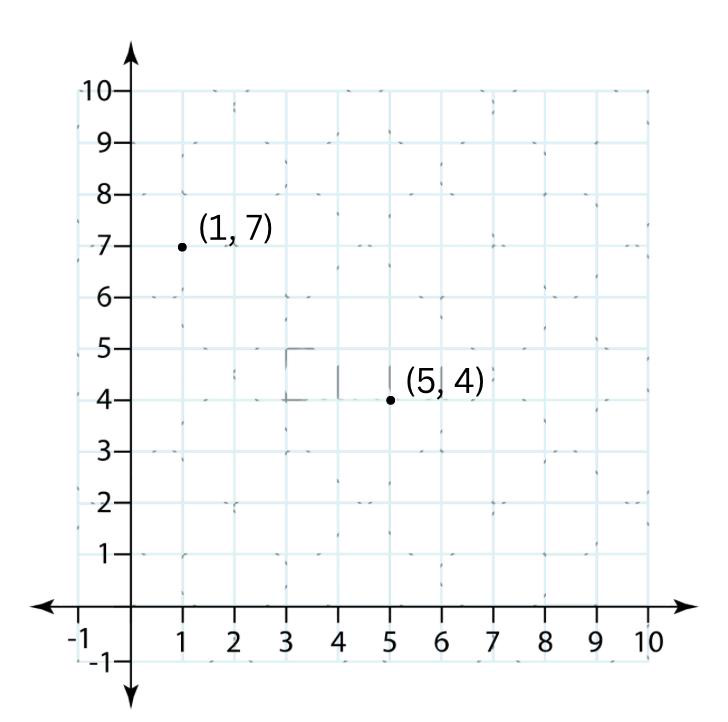
\includegraphics[width=1\linewidth]{vek-mesafe.png}
\newpage
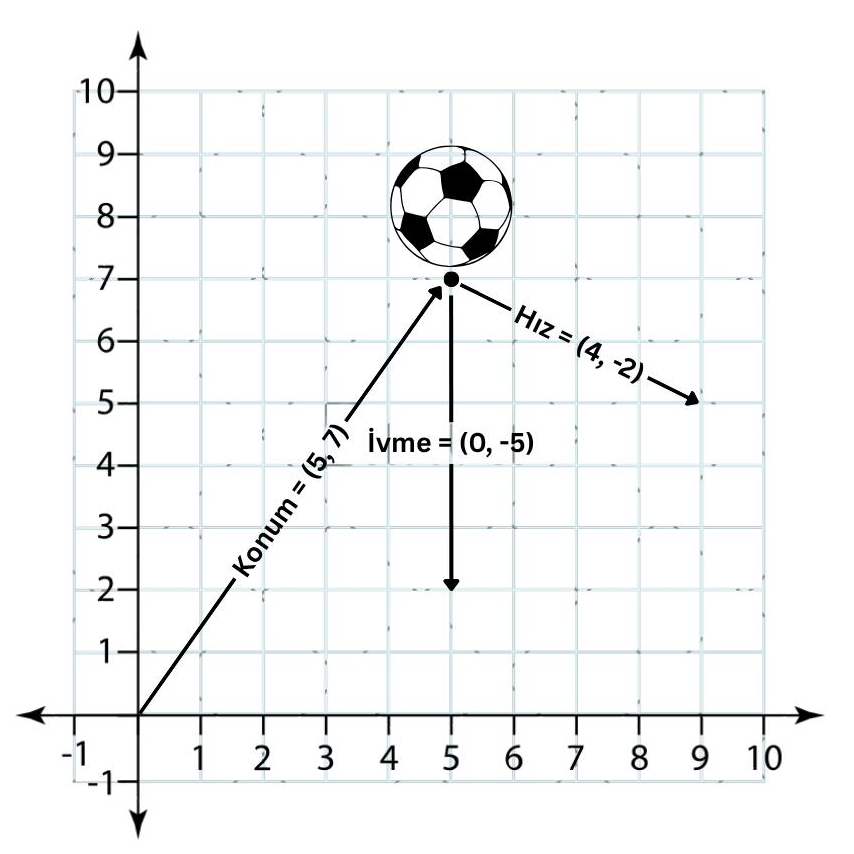
\includegraphics[width=1\linewidth]{vek-konum-hiz-ivme.png}

\begin{itemize}
 \item Konum: Topun başlangıç noktasına göre nerede olduğunu gösterir.
 \item Hız: Top hangi yönde ve ne kadar hızlı hareket ettiğini gösterir.
 
 \item İvme: Topun hareketinin hızlanıp yavaşlayıp değiştiğini belirtir. Burada topa etki eden yer çekimini gösteriyor. 
\end{itemize}


\addcontentsline{toc}{subsection}{Vektör veri yapı}

\veriyapi{v}

\addcontentsline{toc}{subsection}{Vektör fonksiyonların tanımı}
\tasarimtablosu{v+}

\tasarimtablosu{v-}

\tasarimtablosu{v.}

\tasarimtablosu{v*}

\tasarimtablosu{v-mag}


\newpage

\addcontentsline{toc}{section}{Top Oyunu}
\section*{Top Oyunu}
 
\noindent
\addcontentsline{toc}{section}{Top oyunun sahneleri}

\begin{tabular}{| p{16.5cm}  |  }
\hline			
Sahne 1\\
\hline
 \\[50ex]
\hline  
\end{tabular}

\vspace{5ex}
\noindent
\begin{tabular}{| p{16.5cm}  |  }
\hline			
Sahne 2\\
\hline
 \\[50ex]
\hline  
\end{tabular}

\vspace{5ex}
\noindent
\begin{tabular}{| p{16.5cm}  |  }
\hline			
Sahne 3\\
\hline
 \\[50ex]
\hline  
\end{tabular}

\vspace{5ex}
\noindent
\begin{tabular}{| p{16.5cm}  |  }
\hline			
Sahne 4\\
\hline
 \\[50ex]
\hline  
\end{tabular}

\vspace{5ex}
\noindent
\begin{tabular}{| p{16.5cm}  |  }
\hline			
Sahne 5\\
\hline
 \\[50ex]
\hline  
\end{tabular}

\vspace{5ex}

\subsubsection*{Neler değişiyor?}
\begin{tabular}{| p{4cm} | p{11cm} |  }
\hline			
Nesne&Nasıl değişir?\\
\hline
& \\[6ex]
\hline  
& \\[6ex]
\hline  
& \\[6ex]
\hline  
& \\[6ex]
\hline  
& \\[6ex]
\hline  
\end{tabular}


\subsubsection*{Neler değişiyor?}
\begin{tabular}{| p{4cm} | p{11cm} |  }
\hline			
Nesne&Nasıl değişir?\\
\hline
& \\[6ex]
\hline  
& \\[6ex]
\hline  
& \\[6ex]
\hline  
& \\[6ex]
\hline  
& \\[6ex]
\hline  
\end{tabular}

\addcontentsline{toc}{subsection}{Top oyunun verileri}

\subsubsection*{Veriler}
\begin{tabular}{| p{4cm} | p{11cm} |  }
\hline			
Veri ismi&Veri tipi\\
\hline
& \\[2ex]
\hline  
& \\[2ex]
\hline  
& \\[2ex]
\hline  
& \\[2ex]
\hline  
& \\[2ex]
\hline  
& \\[2ex]
\hline  
& \\[2ex]
\hline  
& \\[2ex]
\hline  
& \\[2ex]
\hline  
& \\[2ex]
\hline  
& \\[2ex]
\hline  
& \\[2ex]
\hline  
& \\[2ex]
\hline  
& \\[2ex]
\hline  
& \\[2ex]
\hline  
& \\[2ex]
\hline  
& \\[2ex]
\hline  
& \\[2ex]
\hline  
\end{tabular}
\addcontentsline{toc}{subsection}{Top oyunun veri yapıları}
\veriyapi{ }

\addcontentsline{toc}{subsection}{Top oyunun fonksiyonları}


\tasarimtablosu{nesne-çiz}

\tasarimtablosu{nesne-fizik-güncelle}

%%%add other bouncing ball designs here

\tasarimtablosu{alttan-sek}

\veriyapi{ }

\tasarimtablosu{evren-çiz}

\tasarimtablosu{evren-güncelle}

\addcontentsline{toc}{section}{Benin Oyunum}
\section*{Benin Oyunum}
\noindent
\addcontentsline{toc}{subsection}{Benim Oyunum Sahneleri}

\begin{tabular}{| p{16.5cm}  |  }
\hline			
Sahne 1\\
\hline
 \\[50ex]
\hline  
\end{tabular}

\vspace{5ex}
\noindent
\begin{tabular}{| p{16.5cm}  |  }
\hline			
Sahne 2\\
\hline
 \\[50ex]
\hline  
\end{tabular}

\vspace{5ex}
\noindent
\begin{tabular}{| p{16.5cm}  |  }
\hline			
Sahne 3\\
\hline
 \\[50ex]
\hline  
\end{tabular}

\vspace{5ex}
\noindent
\begin{tabular}{| p{16.5cm}  |  }
\hline			
Sahne 4\\
\hline
 \\[50ex]
\hline  
\end{tabular}

\vspace{5ex}
\noindent
\begin{tabular}{| p{16.5cm}  |  }
\hline			
Sahne 5\\
\hline
 \\[50ex]
\hline  
\end{tabular}

\subsubsection*{Neler değişiyor?}
\begin{tabular}{| p{4cm} | p{11cm} |  }
\hline			
Nesne&Nasıl değişir?\\
\hline
& \\[6ex]
\hline  
& \\[6ex]
\hline  
& \\[6ex]
\hline  
& \\[6ex]
\hline  
& \\[6ex]
\hline  
\end{tabular}

\addcontentsline{toc}{subsection}{Benim oyunumun verı yapıları}
\subsubsection*{Benin Oyunumun veri yapılar}
\begin{tabular}{| p{4cm} | p{11cm} |  }
\hline			
Veri yapı ismi&Veri tipi\\
\hline
& \\[2ex]
\hline  
& \\[2ex]
\hline  
& \\[2ex]
\hline  
& \\[2ex]
\hline  
& \\[2ex]
\hline  
& \\[2ex]
\hline  
& \\[2ex]
\hline  
& \\[2ex]
\hline  
& \\[2ex]
\hline  
& \\[2ex]
\hline  
& \\[2ex]
\hline  
& \\[2ex]
\hline  
& \\[2ex]
\hline  
& \\[2ex]
\hline  
& \\[2ex]
\hline  
& \\[2ex]
\hline  
& \\[2ex]
\hline  
& \\[2ex]
\hline  
\end{tabular}

\veriyapi{ }

\veriyapi{ }

\veriyapi{ }

\veriyapi{ }

\veriyapi{ }

\veriyapi{ }

\veriyapi{ }

\veriyapi{ }

\veriyapi{ }

\veriyapi{ }

\veriyapi{ }

\veriyapi{ }

\veriyapi{ }



\addcontentsline{toc}{subsection}{Benim oyunumun fonksiyonları}

\tasarimtablosu{evren-çiz}

\tasarimtablosu{evren-güncelle}

\tasarimtablosu{evren-güncelle-etkileşim}

\tasarimtablosu{evren-tuş}

\tasarimtablosu{evren-fare}

\tasarimtablosu{ }

\tasarimtablosu{ }

\tasarimtablosu{ }

\tasarimtablosu{ }

\tasarimtablosu{ }

\tasarimtablosu{ }

\tasarimtablosu{ }

\newpage
\addcontentsline{toc}{section}{Cebir ve Evren  için hazır fonksiyonlar}
\section*{Cebir ve Evren  için hazır fonksiyonlar}
\begin{tabular}{| p{4cm} | p{8cm} | p{4cm} |  }
\hline			
Fonksiyon ismi&Giriş veri tip(ler)i&Sonuç veri tipi\\
\hline
\hazirfonkspec{string=?}{string string }{boolean}{İki string eşit ise doğru, yoksa yanlış}
\hazirfonkspec{scale}{imaj sayı }{imaj}{Verilen imaj verilen sayıya göre büyütüp küçültmek}
\hazirfonkspec{image-height}{imaj}{sayı}{Piksel sayısı olarak verilen imajın yüksekliğini hesaplıyor}
\hazirfonkspec{image-width}{imaj}{sayı}{Piksel sayısı olarak verilen imajın genişliğini hesaplıyor}
\hazirfonkspec{rotate}{sayı imaj}{imaj}{Verilen imajı verilen sayıya göre, derece olarak, döndürmek}
\hazirfonkspec{flip-vertical}{imaj}{imaj}{Verilen imajı alt-üst çevirmek}
\hazirfonkspec{flip-horizontal}{imaj}{imaj}{Verilen imajı sağ-sol çevirmek}
\hazirfonkspec{sqr}{sayı}{sayı}{Verilen sayının karesini hesaplıyor}
\hazirfonkspec{sqrt}{sayı}{sayı}{Verilen sayının karekökünü hesaplıyor}
\hazirfonkspec{sine}{sayı}{sayı}{Verilen sayının (derece olarak) sinüsünü hesaplıyor}
\hazirfonkspec{cosine}{sayı}{sayı}{Verilen sayının (derece olarak) kosinüsünü hesaplıyor}
\end{tabular}


 
\section*{Evren için hazır fonksiyonlar}
\begin{tabular}{| p{4cm} | p{8cm} | p{4cm} |  }
\hline			
Fonksiyon ismi&Giriş veri tip(ler)i&Sonuç veri tipi\\
\hline

\hazirfonkspec{place-image/v}{imaj v imaj }{imaj}{Birinci imaj, vektörün belirlediği offset ile sahneye (ikinci imaja) yerleştirmek}
\hazirfonkspec{place-line/v}{v v color imaj }{imaj}{İki vektör arasında olan çizgi verilen color ile ile sahneye (imaja) yerleştirmek}
\hazirfonkspec{place-text/v}{v string color sayı imaj }{imaj}{Vektörün belirlediği yerde verilen metin verilen renkle verilen boyutta sahneye (imaja) yerleştirmek}
\end{tabular}


\end{document}
